\documentclass[12pt]{article}
\usepackage[a4paper, margin=2cm]{geometry}
\usepackage[english]{babel} % To obtain English text with the blindtext package
\usepackage{blindtext}
\usepackage{graphicx} % Required for inserting images
\usepackage{array, multirow} % For extra column formatting
\usepackage{amsmath, amssymb, cancel} %for equation environment
\usepackage{float}
\usepackage{parskip} % For gaps between para
\usepackage{setspace}
\usepackage{pdfpages}
\usepackage{abstract}
\usepackage[export]{adjustbox}
\usepackage{emptypage}
\usepackage{tocloft}
\usepackage[nottoc]{tocbibind}
\usepackage{hyperref, url}
\usepackage[table]{xcolor}
\usepackage{minted}
    \usemintedstyle{monokai}
\usepackage{caption,subcaption}
    \captionsetup{font=footnotesize,labelfont=bf}
\usepackage{tcolorbox}
    \newtcolorbox{mintedbox}{
        colback=backcolour,
        boxrule=0pt,
        sharp corners,
        width=\linewidth,
        left=0pt, right=0pt,
        top=3pt, bottom=3pt
    }
\usepackage{titlesec}

\pagenumbering{arabic}

\cftsetindents{section}{0em}{2em}
\cftsetindents{subsection}{0em}{2em}

\renewcommand\cfttoctitlefont{\hfill\Large\bfseries}
\renewcommand\cftaftertoctitle{\hfill\mbox{}}

\graphicspath{ {./images/} }

\definecolor{blurple}{HTML}{5865F2}
\definecolor{backcolour}{HTML}{272823}

\hypersetup{
    colorlinks=true,
    linkcolor=black,
    urlcolor=black,
    citecolor=blurple,
}

\urlstyle{same}

\renewcommand{\arraystretch}{1.3}

\setcounter{secnumdepth}{5}
\setcounter{tocdepth}{5}
\newcommand\simpleparagraph[1]{%
  \stepcounter{paragraph}\paragraph*{\theparagraph\quad{}#1}}

%%%%%%%%%%%%%%%%%%%%%%%%%%%%%%%%%%%


\title{PHYC20080 Exp.4 Interference}
\author{Joana Adao}
\date{\today}

\begin{document}

\begin{titlepage}
    \begin{center}

        \begin{figure}[ht]
            
\includegraphics[width=\textwidth]{UCDLogo.png}
        \end{figure}
        
        \begin{figure}
            \centerline{
\includegraphics[width=\paperwidth]{UCDBanner.png}}
        \end{figure}

        \vspace{4cm}

        {\LARGE \bfseries PHYC20080 Fields, Waves and Light}\\
        \vspace{0.75cm}
        {\Large Experiment No.4 Interference and Diffraction}
        
        \vspace{1cm}
    
    {\Large \textbf{25 March 2025}}
    
    \vspace{2cm}
    
    {\large \textbf{by Joana C.C. Adao (Student No. 23311051)}}\\
    \vspace{.25cm}
    {\large With Beau Etac}\\
    \vspace{0.25cm}
    {\large Tuesday 16.00-18.00 Slot}\\
    {\large Nicki (Coordinator)}

    \end{center}
    
   \clearpage

\end{titlepage}


\tableofcontents
\thispagestyle{empty}

\newpage

\begin{abstract}
\addtocontents{toc}{\protect\contentsline{section}{\textbf{Abstract}}{\hfill}{}}
\thispagestyle{empty}



 
\end{abstract}
\newpage

%%%%%%%%%%%%%%%%%%%%%%%%%%%%%%%%%%%

\setcounter{page}{1}
\section{Theory} \label{sec:1}

\subsection{Wave Nature of Light}

The wave nature of light was first demonstrated through slit experiments, in which light displayed diffraction (see §\ref{sec:1.2}) and interference (see §\ref{sec:1.3}) behaviours. Therefore, it was concluded that light
is a \textit{transverse, eletromagnetic wave}. The transverse wave nature of light can be demonstrated through polarisation of the wave \cite{natureoflight}.

\subsection{Diffraction} \label{sec:1.2}

Diffraction is the way light waves "bend" around barriers, such as a corner or through an opening, and consequently spread out. The diffraction patterns formed are parallel lines.
Diffraction is a specialised case of light scattering, such that when light encounters an object with regularly repeating openings (such as diffraction gratings) it produces an orderly diffraction pattern.
\cite{diffraction1}. 

\subsubsection{Fresnel Diffraction}

Fresnel diffraction is a near-field approximation of the Kirchoff or Rayleigh-Sommerfield diffraction integral, which describes how a wave propagates after encountering an obstacle. Fresnel's approximation
specifically pertains to when the recording screen is close in distance to the slits. Typically, this leads to more complex interference patterns (see Figure \ref{fig:2}) \cite{fresnelfraunhofer}.

\begin{figure}[H]
    \centering
    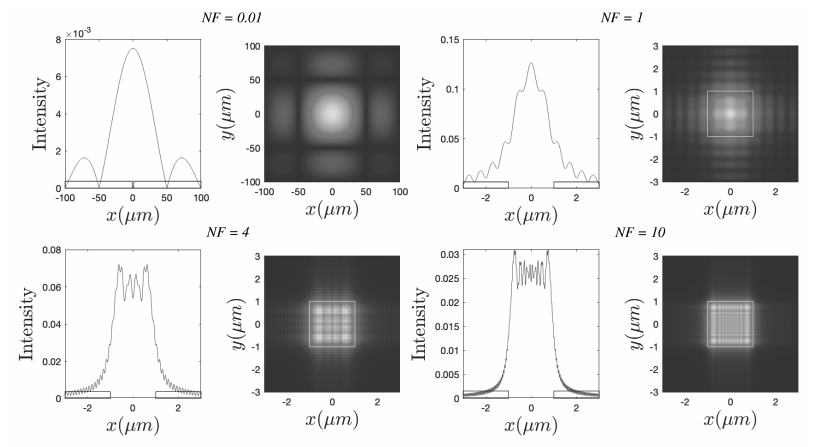
\includegraphics[width=.85\textwidth]{fresnel patterns.png}
    \caption{Example of intensities of Fresnel fields of a square opening, shown as contours and in cross-section for different distances, which increase from the lower right to the upper left.
    The upper left pattern is equal to the Fraunhofer pattern \protect\cite{fresnelfraunhofer}.}
    \label{fig:2}
\end{figure}

The minima condition for Fresnel diffraction is given as,

\vspace{-2ex}
\begin{gather*}
    \frac{x}{z} = (2m + 1) \frac{\lambda}{2a}
\end{gather*}

and maxima on,

\vspace{-2ex}
\begin{gather*}
    \frac{x}{z} = m \frac{\lambda}{a}
\end{gather*}

with $m$ as an integer of the order of the maxima/minima, $z$ as the distance between the screen and the opening (slit), $\lambda$ as the wavelength of light, $a$ as the half-width of the slit ($2a$ being the full width),
and $x$ as the distance of a point from the centre of the diffraction pattern on the screen \cite{fresnelfraunhofer}.

\subsubsection{Fraunhofer Diffraction}

Fraunhofer diffraction is a far-field approximation of the Kirchoff or Rayleigh-Sommerfield diffraction integral. Fraunhofer's approximation specifically pertains to when the recording screen is a considerable distance from the oopening (slit) \cite{fresnelfraunhofer}.
The resuting interference patterns are most associated with the traditional single slit (see §\ref{sec:1.4}) and double slit (see §\ref{sec:1.5}) experiments.

The intenisty pattern of a single-slit diffraction experiment is given by,

\vspace{-2ex}
\begin{gather*}
    I(\theta) = I_0 [sinc(\beta)]^2 \qquad , \qquad I(\theta) \propto \left( \frac{sin(\beta)}{\beta} \right)
\end{gather*}

where

\vspace{-2ex}
\begin{gather*}
    \beta \equiv \frac{ak sin \theta}{2} = \frac{a \pi sin \theta}{\lambda} \qquad , \qquad k = \frac{2 \pi}{\lambda}
\end{gather*}

where $I$ is the intensity, $a$ is the slit width, $k$ is the wavenumber, $\theta$ is the angle the fringe makes from the central axis, $\lambda$ is the wavelegnth \cite{fraunhofer}.

\subsection{Interference} \label{sec:1.3}

Interference, when in reference to light and optics, occurs when two or more light beams collide and are superimposed. Interference occurs when spatial and temporal phases overlap for both light beams,
the phase is \textit{coherent}, and the light has non-orthogonal polarisation states \cite{Paschotta_2005_interference}.

\subsubsection{Laser Properties for Interference}

Lasers are \textbf{highly monochromatic and coherent} which allows for stable interference patterns to be formed, making it much simpler to read and see the interference fringes.

\paragraph{Monochromaticity} \label{sec:1.3.1} \leavevmode\\
\vspace{-3ex}

For stable interference, the source itself must be stable such that the light is emitted at a single wavelength \cite{princelaser}.
Any variation in wavelength would cause the fringes to become "blurred". The laser being monochromatic ensures the fringes remain sharp and stable (well-defined).

\begin{figure}[H]
    \centering
    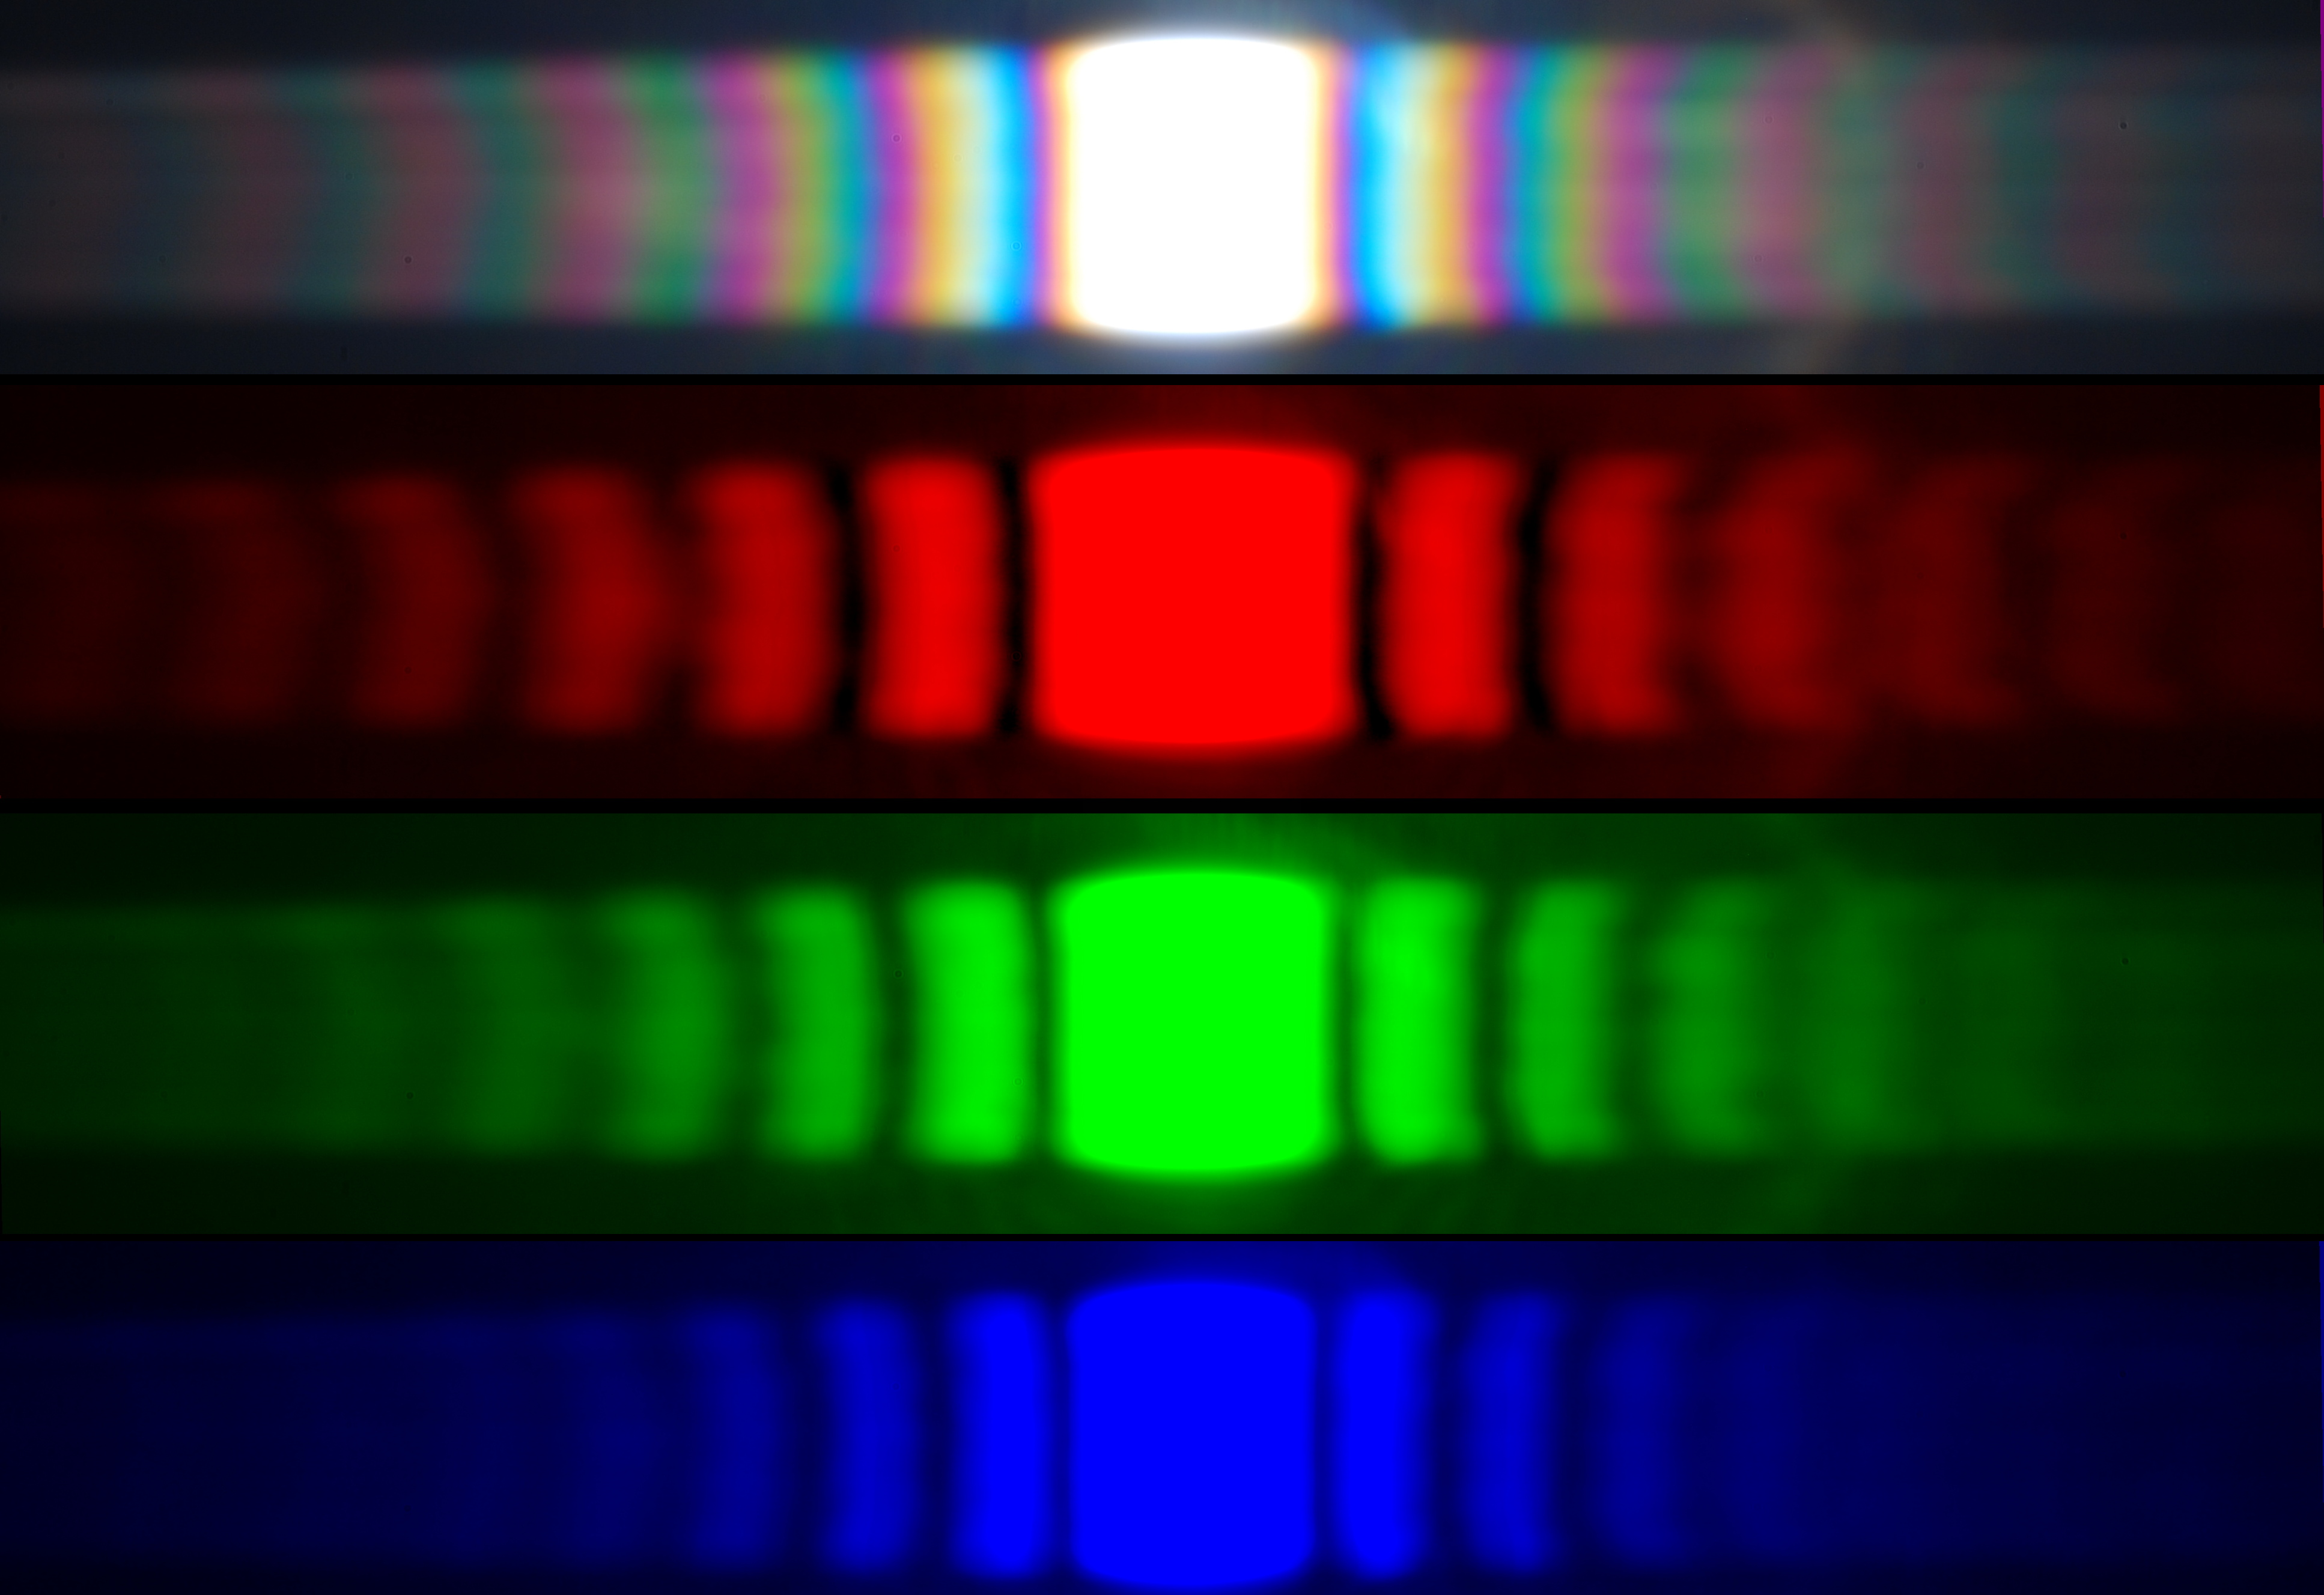
\includegraphics[width=.5\textwidth]{interference patterns.jpg}
    \caption{\centering Double slit experiment for different coloured lights (white, red, green, blue) \protect\cite{holoimg2}.}
    \label{fig:4}
\end{figure}

As can be seen in Figure \ref{fig:4}, the interference patterns from the monochromatic light sources (red, green, blue) appear much sharper than the "blurred" interference pattern of the white light (top)
due to the range of wavelengths present in white light. White light appears "blurry" due to the wavelength of each colour being diffracted at a alightly different angle.

\paragraph{Coherence} \label{sec:1.3.2} \leavevmode\\
\vspace{-3ex}

For there to be stable interference, the light source must have a fixed phase relationship at different points in time and/or space \cite{wolf2007introduction}.
This property ensures that light beams maintain a consistent phase difference, allowing them to interfere and create the fringes of greater and lesser amplitudes
\cite{Born_Wolf_Bhatia_Clemmow_Gabor_Stokes_Taylor_Wayman_Wilcock_1999}.

\begin{figure}[H]
    \centering
    \begin{subfigure}[b]{.45\textwidth}
        \centering
        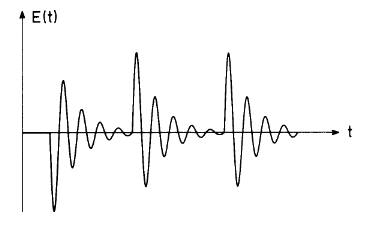
\includegraphics[width=\linewidth]{incoherent source.png}
        \caption{\centering Incoherent lamp light source}
        \label{fig:5a}
    \end{subfigure}
    \hspace{-.5em}
    \begin{subfigure}[b]{.45\textwidth}
        \centering
        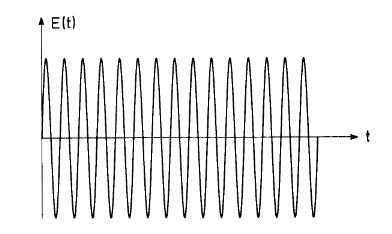
\includegraphics[width=\linewidth]{coherent source.png}
        \caption{\centering Coherent laser light source}
        \label{fig:5b}
    \end{subfigure}
    \caption{(a) The electric field strength E(t) of light of a lamp consists of uncorrelated individual wave tracks.
    (b) Laser light consists of a single coherent very strong wave track. \protect\cite{haken1986laser}.}
    \label{fig:5}
\end{figure}

A graphical representation of an incoherent (\ref{fig:5a}) and a coherent (\ref{fig:5b}) can be seen in Figure \ref{fig:5} above. Visually, it can be understood why a coherent
source is necessary for the production of stable interference fringe patterns.

\subsection{Single Slit Experiment} \label{sec:1.4}

For a single slit experiment the central maximum will be much larger than the adjacent and subsequent maxima, with the intensity decreasing rapidly from the centre. The interference patterns form
as the wave arrives either in or out of phase to a common location (the screen). The central maximum is so bright because majority of the light will arrive straight-on and therefore in phase \cite{urone2012collegesingle}.

The following equation describes the minima of the fringe pattern,

\vspace{-2ex}
\begin{gather}
    a sin \theta = m \lambda
\end{gather}

where $a$ is the slit width, $\theta$ is the angle, $m$ is an integer, and $\lambda$ is the wavelength. It can then be found that the slit width is (for $\theta$ small $\approx sin \theta$) \cite{UCDinterference}:

\vspace{-2ex}
\begin{gather}
    a = \lambda \frac{D}{Y}
\end{gather}

with $D$ as the distance from the pattern to the slit, and $Y$ as the distance from the central maximum to the first minimum.

\subsection{Double Slit (Young's) Experiment} \label{sec:1.5}

Thomas Young was the first to prove that light was indeed also a wave by means of the double slit experiment (see Figure \ref{fig:1}). Light must interact somthing small, such as the small opening of the slits, in order to
exhibit wave-like behaviour and the light must also be coherent \cite{urone2012collegedouble}.

\begin{figure}[H]
    \centering
    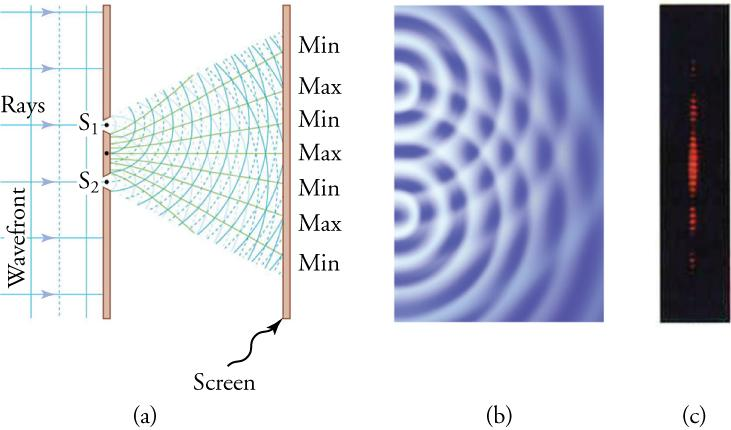
\includegraphics[width=.7\textwidth]{diffraction pattern.jpg}
    \caption{ Double slits produce two sources that interfere. (a) Diffraction of light as it encounters a barrier, forming dark and bright regions of destructive and constructive interference, respectively.
    (b) Double-slit interference pattern for diffracted light. (c) Pattern seen when light falls onto a screen. \protect\cite{urone2012collegedouble}}
    \label{fig:1}
\end{figure}

The equation for the double slit experiment imply there are a series of dark and bright fringes formed due to destructive and constructive interference of the light. The cloesr the slits are to each other, the more spread out the fringes will be (see Figure \ref{fig:3}).
This can be observed by examining the equation \cite{urone2012collegedouble},

\vspace{-2ex}
\begin{gather}
    d sin \theta = n \lambda
\end{gather}

where $n$ is an integer, $\theta$ is the angle, $\lambda$ is the wavelength, and $d$ is the distance between the slits.

\begin{figure}[H]
    \centering
    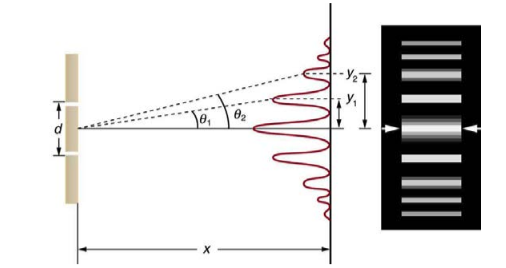
\includegraphics[width=.7\textwidth]{youngs slit.png}
    \caption{\centering The interference pattern for a double slit \protect\cite{urone2012collegedouble}.}
    \label{fig:3}
\end{figure}

When the angle is small, the approximation $sin \theta \approx \theta$ may be used to get

\vspace{-2ex}
\begin{gather}
    n \lambda \approx d \theta
\end{gather}

therefore the angular separation between adjacent maxima is

\vspace{-2ex}
\begin{gather}
    \frac{\lambda}{d} = \frac{y}{D}
\end{gather}

where $y$ is the linear separation between adjacent maxima, and $D$ is the distance from the pattern to the slit \cite{UCDinterference}.

\subsection{Applications of Interference and Diffraction}

\textbf{Holography} is based on \textit{interference}

\textbf{Spectroscopy} is based on \textit{diffraction}

\section{Methodology} \label{sec:2}

\subsection{Single Slit Experiment Method} \label{sec:2.1}



\subsection{Double Slit (Young's) Experiment Method} \label{sec:2.2}




\section{Results and Discussion} \label{sec:3}

\subsection{Single Slit Experiment Results}



\subsection{Double Slit (Young's) Experiment Results}



\section{Conclusion} \label{sec:4}



\newpage

%%%%%%%%%%%%%%%%%%%%%%%%%%%%%%%%%%%

\bibliographystyle{IEEEtran}
\bibliography{References} \label{sec:ref}

\vspace{1.5cm}

\listoffigures


\end{document}